%!TEX root = ../lab.tex

\section{ХОД РАБОТЫ}

\subsection{Текст задания}

Заданы три числа D, M, Y, которые обозначают число, месяц и год. Найти номер N этого дня с начала года (високосные года --- это те, у которых номер делится на 400, и те, у которых номер делится на четыре, но не делится на 100).

\subsection{Особенности разработанной программы}

Разработанная программа предоставляет пользователю удобный в использовании интерфейс, защищённый от попыток переполнения и некорректного ввода информации.

На рисунке~\ref{lst:init} представлены переменные, участвующие во взаимодействии с пользователем, а также массив из 12 чисел, соответствующих количеству дней в соответствующем месяце.

\begin{lstlisting}[caption=Объявление переменных и инициализация массива,label=lst:init]
  int d, m, y;
  int result;
  int days[12] = {31, 29, 31, 30, 31, 30, 31, 31, 30, 31, 30, 31};  
\end{lstlisting}

Часть исходного кода, обеспечивающего вычисление количества дней, прошедших с начала года, изображена на рисунке~\ref{lst:main_function}.

\begin{lstlisting}[caption=Вычисление количества дней,label=lst:main_function]
  int i = 0;
  while (i < m-1) {
    result += days[i];
    i++;
  }
  result += d;
\end{lstlisting}

На рисунке~\ref{fig:image1} представлен пример работы разработанной программы: пользователь выбирает пункт меню <<Enter date>>, затем ему предлагается ввести год, месяц и день соответственно. При попытке ввода дня пользователь допускает ошибку и система сообщает ему об этом, указывая верный диапазон значений для конкретного месяца. После этого пользователь повторно вводит день и программа печатает результат. Пользователь завершает работу с программой, выбрав пункт меню <<Quit>>.

\begin{figure}[htbp]
  \centering
  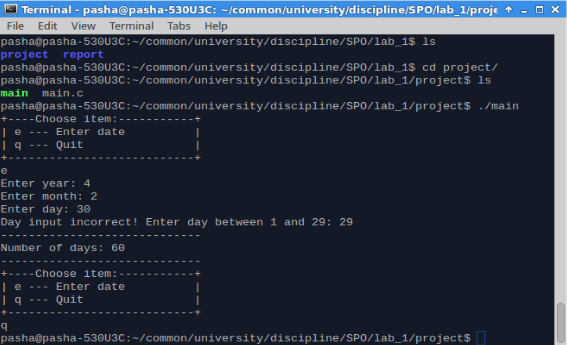
\includegraphics[width=150mm,height=92mm]{img/image1}
  \caption{Пример работы программы}\label{fig:image1}
\end{figure}

Исходный текст программы расположен в приложении А.

\newpage